\documentclass[12pt,xcolor=table,aspectratio=169]{beamer}
\usetheme{Frankfurt}
\usecolortheme{rose}
\usepackage{amsthm}
\usepackage{amsmath}
\usepackage{bbm}
\usepackage{amsfonts}
\usepackage{amssymb}
\usepackage{graphicx}
\usepackage{hyperref}
\usepackage[flushleft]{threeparttable}
\usepackage{tabularx}
\usepackage{booktabs}
\usepackage{siunitx}
\usepackage{tikz}
\usetikzlibrary{decorations.pathreplacing,angles,quotes}
%\usepackage{enumitem}% http://ctan.org/pkg/enumitem

%set up course and number

\newcommand{\ClassName}{TBD}
\newcommand{\ClassNumber}{TBD}
\newcommand{\Topic}{TBD}

% Some optional colors. Change or add as you see fit.
%---------------------------------------------------
 \definecolor{ualbertagreen}{HTML}{007C41}
\definecolor{ualbertagold}{HTML}{FFDB05}

\definecolor{calloutgrey}{HTML}{D9D9D9}


%set fonts
\setbeamerfont{subtitle}{size=\large,shape=\scshape,series=\bfseries}
\setbeamerfont{title}{size=\Large,shape=\scshape,series=\bfseries}
\setbeamerfont{author}{size=\large}
\setbeamerfont{date}{size=\large}
\setbeamerfont{caption}{size=\scriptsize}


% Some optional color adjustments to Beamer. Change as you see fit.
%------------------------------------------------------------------
\setbeamercolor{frametitle}{fg=ualbertagreen,bg=white}
\setbeamercolor{title}{fg=ualbertagreen,bg=white}
\setbeamercolor{author}{fg=ualbertagreen,bg=white}
\setbeamercolor{date}{fg=ualbertagreen,bg=white}
\setbeamercolor{local structure}{fg=ualbertagreen}
\setbeamercolor{section in toc}{fg=ualbertagreen,bg=white}
% \setbeamercolor{subsection in toc}{fg=ualbertagreen,bg=white}
\setbeamercolor{footline}{fg=ualbertagreen!50, bg=white}

% definition boxes
\setbeamercolor{block title}{bg=ualbertagreen,fg=white}
\setbeamercolor{block body}{parent=normal text,use=block title,bg=calloutgrey}
%\setbeamercolor{block body}{parent=normal text,use=block title,bg=block title.bg!30!bg}


\setbeamercolor{upper separation line head}{bg=ualbertagreen}
\setbeamercolor{lower separation line head}{bg=ualbertagold}
\setbeamercolor{middle separation line head}{bg=ualbertagold}
\setbeamercolor{frametitle}{fg=ualbertagreen,bg=white}



\setbeamercolor{section in head/foot}{bg=white,fg=ualbertagreen}
\setbeamercolor{author in head/foot}{bg=white,fg=ualbertagreen}
\setbeamercolor{date in head/foot}{bg=white,,fg=ualbertagreen}
\setbeamercolor{title in head/foot}{bg=white,fg=ualbertagreen}

\setbeamercolor{headline}{bg=white,fg=ualbertagreen}




\setbeamercolor*{middle separation line head}{bg=ualbertagreen}
\setbeamercolor*{alerted text}{fg=ualbertagreen}
\setbeamercolor*{example text}{fg=black}
\setbeamercolor*{structure}{fg=black}


\let\Tiny=\tiny



\logo{
   %\ifnum\insertpagenumber>1
   \tikz [remember picture,overlay]
    \node[yshift=.3cm,xshift=1.5cm] at (current page.south west)
        %or: (current page.center)
        {
\includegraphics[width=1in]{../images/UA-ASB-COLOUR.png}};
    %\fi
%
\includegraphics[height=0.8cm]{../images/UA-ASB-COLOUR.png}\vspace{220pt}
}


\setbeamertemplate{title page}{%
  \vbox{}
    \vspace{.5cm}% NEW
  \begingroup
    \centering
    \begin{beamercolorbox}[sep=8pt,center]{title}
      \usebeamerfont{title}\ClassNumber: \ClassName\par%
      \usebeamerfont{title}\inserttitle\par%
     \ifx\insertsubtitle\@empty%
      \else%
        \vskip0.05em%
        {\usebeamerfont{subtitle}\usebeamercolor[fg]{subtitle}\insertsubtitle\par}%
      \fi%
    \end{beamercolorbox}%
    \begin{beamercolorbox}[sep=8pt,center]{author}
      \usebeamerfont{author}\insertauthor
    \end{beamercolorbox}
    \begin{beamercolorbox}[sep=8pt,center]{institute}
      \usebeamerfont{institute}\insertinstitute
    \end{beamercolorbox}

    \vspace{0.5cm}% NEW
    \begin{beamercolorbox}[sep=8pt,center]{date}
      \usebeamerfont{date}\insertdate
    \end{beamercolorbox}\vskip0.05em

      \endgroup
  %\vfill
}


\setbeamertemplate{frametitle}{%
    \insertframetitle\par\vskip-10pt
}



\renewcommand{\ClassName}{Business Economics, Organization and Management}
\renewcommand{\ClassNumber}{BUEC 311}

\setbeamertemplate{headline}{%
\leavevmode%
 \hbox{%
    \begin{beamercolorbox}[wd=\paperwidth,ht=5ex,dp=0ex]{white}%
    \usebeamerfont{headline}\hskip6pt\ClassNumber: \inserttitle\par%
    \insertsectionnavigationhorizontal{\paperwidth}{}{\hskip0pt plus1filll}
    \end{beamercolorbox}%
  }
}

\defbeamertemplate*{footline}{my footline}{%
    \ifnum\insertpagenumber=1
        \Tiny{%
            \hfill%
		\vspace*{1pt}%
            %\insertframenumber/\inserttotalframenumber \hspace*{0.1cm}%
            \newline%
            \color{ualbertagold}{\rule{\paperwidth}{0.4mm}}\newline%
            \color{ualbertagold}{\rule{\paperwidth}{.4mm}}%
        }
  \else%
        \Tiny{%
            \hspace{.66\paperwidth}
            %\vspace{25pt}
            \insertframenumber/\inserttotalframenumber
            \newline%
            \color{ualbertagold}{\rule{\paperwidth}{0.4mm}}\newline%
            \color{ualbertagold}{\rule{\paperwidth}{.4mm}}%
        }%
    \fi%
}


\newenvironment{itemize*}%
  {\begin{itemize}%
    \setlength{\itemsep}{0pt}%
    \setlength{\parskip}{0pt}}%
  {\end{itemize}}


\title{
Pricing with Market Power
}

\date{Fall 2020}

\begin{document}

\frame{
	\titlepage
}

\frame{
	\frametitle{Outline}
	\begin{enumerate}
	\item Price Discrimination
	\item[]
	\item Perfect Price Discrimination
	\item[]
	\item Group Price Discrimination
	\item[]
	\item Nonlinear Price Discrimination
	\item[]
	\item Two-Part Pricing
	\item[]
	\item Bundling
	\item[]
	\item Peak-Load Pricing
	\item[]
	\item Pricing in Practice
	\end{enumerate}
}

\frame{
	\frametitle{Outline}
	\begin{enumerate}
	\item \alert{Price Discrimination}
	\item[]
	\item Perfect Price Discrimination
	\item[]
	\item Group Price Discrimination
	\item[]
	\item Nonlinear Price Discrimination
	\item[]
	\item Two-Part Pricing
	\item[]
	\item Bundling
	\item[]
	\item Peak-Load Pricing
	\item[]
	\item Pricing in Practice
	\end{enumerate}
}

\frame{
	\frametitle{1. Price Discrimination}
	\begin{itemize}
	\item Should firms charge all of their customers the same price?
	\end{itemize}
}

\frame{
	\frametitle{1. Price Discrimination}
	\begin{itemize}
	\item \underline{Price discrimination} occurs when a firm charges different prices for a good or service.
	\item[]
	\item \underline{Idea}: Exploit the fact that, for almost any good or service, some consumers are willing to pay more for a good/service than others.
	\item[]
	\item Price discrimination increases profit above level achieved with uniform pricing via two channels:
		\begin{enumerate}
		\item Higher prices for some.
			\begin{itemize}
			\item Price discrimination can extract additional CS from consumers who place a high value on a good/service.
			\end{itemize}
		\item New customers.
			\begin{itemize}
			\item Firms can also sell to new customers who would not be willing to pay profit-maximizing uniform price.
			\end{itemize}
		\end{enumerate}
	\end{itemize}
}

\frame{
	\frametitle{1. Price Discrimination}
	\begin{figure}
	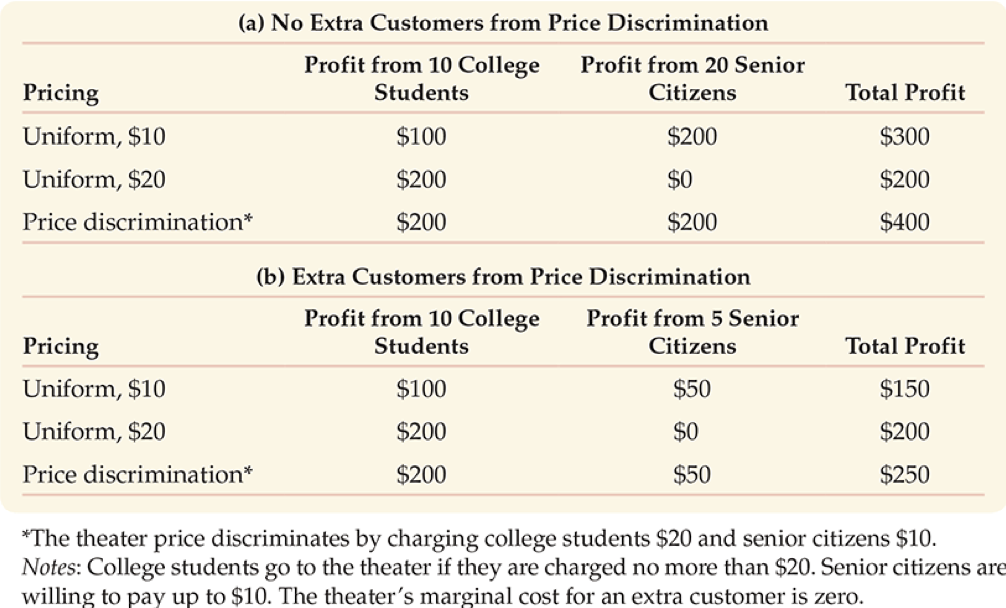
\includegraphics[scale=0.66]{../images/price_disc/tickets.png}
	\caption{Pricing of Theatre Tickets}
	\end{figure}	
}

\frame{
	\frametitle{1. Price Discrimination}
	\begin{itemize}	
	\item To price discriminate, the firm must:
		\begin{enumerate}
		\item Have market power.
			\begin{itemize}
			\item Monopolist, oligopolist, or monopolistically competitive firm may be able to price discriminate.
			\item Perfectly competitive firm cannot.
			\end{itemize}
		\item[]
		\item Identify groups with different price sensitivities.
			\begin{itemize}
			\item Firm must identify demand differences across consumers.
			\end{itemize}
		\item[]
		\item Prevent resale.
			\begin{itemize}
			\item This is usually the biggest obstacle to price discrimination.
			\item Why?
			\end{itemize}
		\end{enumerate}
	\end{itemize}
}

\frame{
	\frametitle{1. Price Discrimination}
	\begin{itemize}
	\item Resale is easier in some industries than others.
	\item[]
	\item Managers can take actions to make resale more difficult.
		\begin{itemize}
		\item Raise transaction costs.
			\begin{itemize}
			\item E.g. require photo id for use of low priced tickets.
			\end{itemize}
		\item Require contracts forbidding resale.
			\begin{itemize}
			\item E.g. Student discounts on computers/software.
			\end{itemize}
		\item Void warranties if purchase from unauthorized retailer.
			\begin{itemize}
			\item E.g. Nikon and international resale; Costco and watches.
			\end{itemize}
		\end{itemize}
	\end{itemize}
}

\frame{
	\frametitle{1. Price Discrimination}
	\begin{itemize}
	\item While it can be profit maximizing for a firm with market power to price discriminate, not all price difference are due to price discrimination.
	\item[]
	\item Some price differences are due to differences in costs.
		\begin{itemize}
		\item E.g. Newsstand vs. subscription price for magazines.
		\end{itemize}
	\end{itemize}
}

\frame{
	\frametitle{1. Price Discrimination}
	\begin{itemize}
	\item Three main types of price discrimination:
		\begin{itemize}
		\item \underline{Type 1}: Perfect Price Discrimination (1st degree price discrimination)
			\begin{itemize}
			\item The firm sells each unit that the maximum amount any customer is willing to pay.
			\item Price differs across consumers, and may even differ for a given consumer.			
			\end{itemize}
		\item[]
		\item \underline{Type 2}: Group Price Discrimination (3rd degree price discrimination)
			\begin{itemize}
			\item The firm charges each group of customers a different price, but it does not charge different prices within the group.
			\end{itemize}
		\item[]
		\item \underline{Type 3}: Nonlinear Price Discrimination (2nd degree price discrimination)
			\begin{itemize}
			\item The firm charges a different price for large purchases than for small quantities so that the price paid varies according to the quantity purchased.
			\end{itemize}
		\end{itemize}
	\end{itemize}
}

\frame{
	\frametitle{Outline}
	\begin{enumerate}
	\item Price Discrimination
	\item[]
	\item \alert{Perfect Price Discrimination}
	\item[]
	\item Group Price Discrimination
	\item[]
	\item Nonlinear Price Discrimination
	\item[]
	\item Two-Part Pricing
	\item[]
	\item Bundling
	\item[]
	\item Peak-Load Pricing
	\item[]
	\item Pricing in Practice
	\end{enumerate}
}

\frame{
	\frametitle{2. Perfect Price Discrimination}
	\begin{itemize}
	\item A firm with market power that can prevent resale and has full information about its customers' willingness to pay price discriminates by selling each unit at the \textit{reservation price}.
	\end{itemize}
	\begin{definition}[Reservation Price]
	The maximum amount any consumer would pay for a good.
	\end{definition}
	\begin{itemize}
	\item Given the demand curve indicates willingness to pay, the reservation price is given by the height of the demand curve at each output level.
	\item[]
	\item Hence, a perfectly price-discriminating firm's marginal revenue is the same as its price.
		\begin{itemize}
		\item This means the firm's marginal revenue curve is the same as its demand curve.
		\end{itemize}
	\end{itemize}
}	

\frame{
	\frametitle{2. Perfect Price Discrimination}
	\begin{figure}
	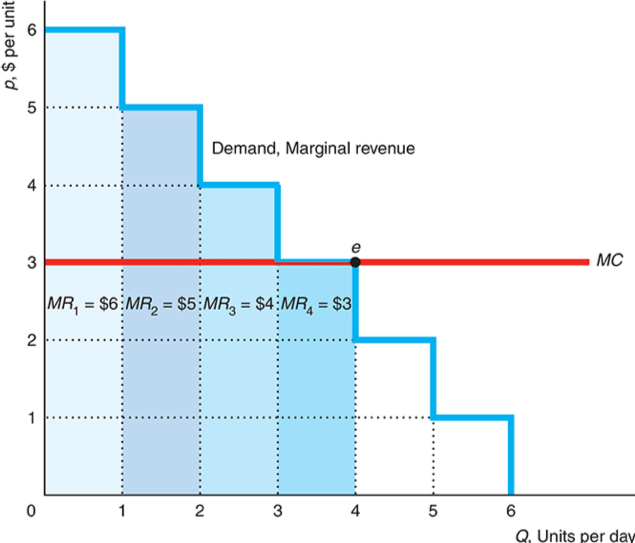
\includegraphics[scale=0.66]{../images/price_disc/ppd_step.png}
	\end{figure}
}

\frame{
	\frametitle{2. Perfect Price Discrimination}
	\begin{itemize}
	\item Perfect price discrimination is efficient because it maximizes the sum of consumer surplus and producer surplus.
	\item[]
	\item But \underline{all of the surplus goes to the firm}; consumer surplus is zero.
	\item[]
	\item Consumer surplus is greatest with competition, lower with a single-price monopoly, and eliminated by perfect price discrimination.
	\end{itemize}
}

\frame{
	\frametitle{2. Perfect Price Discrimination}
	\begin{figure}
	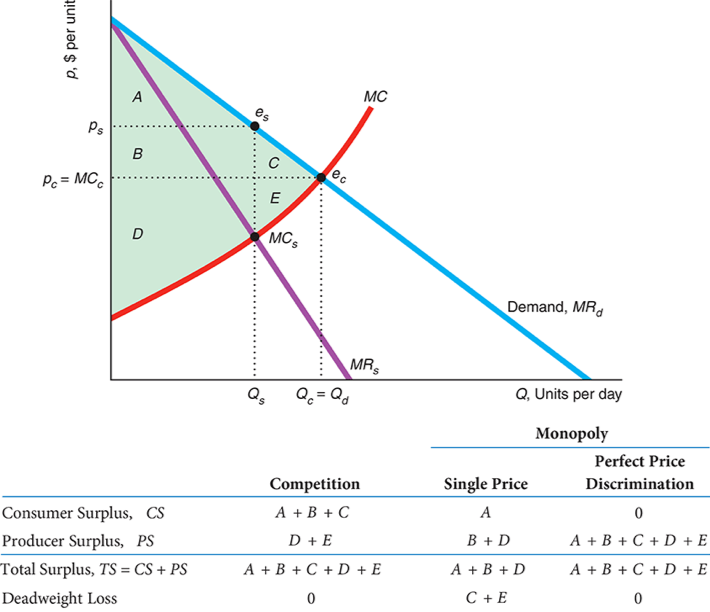
\includegraphics[scale=0.66]{../images/price_disc/ppd.png}
	\end{figure}
}

\frame{
	\frametitle{2. Perfect Price Discrimination}
	\begin{itemize}
	\item Perfect price discrimination is rarely fully achieved in practice.
	\item[]
	\item Firms can still increase profits with imperfect individual price discrimination.
		\begin{itemize}
		\item Idea: charge individual-specific prices to different consumers, which may or may not be the consumers' reservation prices.
		\end{itemize}
	\item[]
	\item Historically, it was difficult to gather information on consumer reservation prices due to high transaction costs, but this is changing.
		\begin{itemize}
		\item Change largely due to computer technology.
		\item Hotels, car/truck rental companies, cruise lines, airlines, and other firms are increasingly using individual price discrimination.
		\end{itemize}
	\end{itemize}
}

\frame{
	\frametitle{Outline}
	\begin{enumerate}
	\item Price Discrimination
	\item[]
	\item Perfect Price Discrimination
	\item[]
	\item \alert{Group Price Discrimination}
	\item[]
	\item Nonlinear Price Discrimination
	\item[]
	\item Two-Part Pricing
	\item[]
	\item Bundling
	\item[]
	\item Peak-Load Pricing
	\item[]
	\item Pricing in Practice
	\end{enumerate}
}

\frame{
	\frametitle{3. Group Price Discrimination}
	\begin{itemize}
	\item Group price discrimination occurs when potential customers are divided into two or more groups with different prices for each group (and a single price within a group).
	\item[]
	\item Two conditions for group price discrimination.
		\begin{enumerate}
		\item Consumer groups must differ via an observable characteristic (age, location, etc).
		\item The firm must have market power, be able to identify groups with different reservation prices, and prevent resale.
		\end{enumerate}
	\end{itemize}
}

\frame{
	\frametitle{3. Group Price Discrimination: 2 Group Example}
	\begin{itemize}
	\item Warner Brothers, a legal monopoly by copyright, produces and sells \textit{Harry Potter and the Deathly Hallows, Part 2} on DVD in various countries.
	\item[]
	\item Warner Bros. engaged in group price discrimination by charging different prices in different countries.
		\begin{itemize}
		\item Resale not possible because DVDs have incompatible formats.
		\end{itemize}
	\item[]
	\item In this case, Warner Bros has a common marginal cost, and maximizes profit by acting like a traditional monopoly in each market.
		\begin{itemize}
		\item Differences in prices across countries reflects differences in demand.
		\end{itemize}
	\end{itemize}
}

\frame{
	\frametitle{3. Group Price Discrimination: 2 Group Example}
	\begin{figure}
	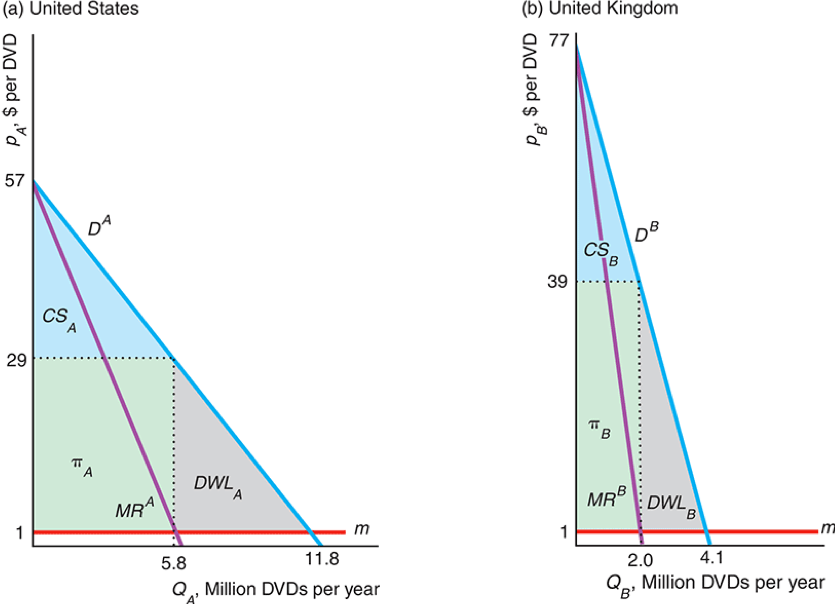
\includegraphics[scale=0.66]{../images/price_disc/gpd.png}
	\end{figure}
}

\frame{
	\frametitle{3. Group Price Discrimination: 2 Group Example}
	\begin{itemize}
	\item With two groups ($A$ and $B$), and a common marginal cost, a firm engaged in group price discrimination produces where:
		\begin{align*}
		MR^{A} = MC = MR^{B}
		\end{align*}
	\item Recall that for a profit maximizing monopolist: $MR = p[1+1/\varepsilon]$. Thus:
		\begin{align*}
		MR^{A} = p_{A}[1+1/\varepsilon_{A}] = MC = p_{B}[1+1/\varepsilon_{B}] = MR^{B}
		\end{align*}
		Which implies:
		\begin{align*}
		\frac{p_{B}}{p_{A}} = \frac{[1+1/\varepsilon_{A}]}{[1+1/\varepsilon_{B}]}
		\end{align*}
		That is, the ratio of prices depends on the elasticity of demand in the two markets.
	\end{itemize}
}

\frame{
	\frametitle{3. Group Price Discrimination}
	\begin{itemize}
	\item Key issue for group price discrimination: dividing customers into groups.
	\item[]
	\item How might a firm do this?
	\end{itemize}
}

\frame{
	\frametitle{3. Group Price Discrimination}
	\begin{itemize}
	\item Two possible approaches:
		\begin{enumerate}
		\item Divide based on \underline{observable characteristics}.
			\begin{itemize}
			\item Idea: Some characteristics are associated with high/low reservation prices or demand elasticities.
			\end{itemize}
		\item[]
		\item Divide based on \underline{actions}.
			\begin{itemize}
			\item Idea: Allow people to self select on the basis of the value of time.
			\end{itemize}
		\end{enumerate}
	\end{itemize}
}

\frame{
	\frametitle{3. Group Price Discrimination}
	\begin{itemize}
	\item $CS$ is greater and more output is produced with perfect competition than with group price discrimination.
		\begin{itemize}
		\item Group price discrimination transfers some of the competitive $CS$ to the firm as additional profit, and causes deadweight loss due to reduced output.
		\end{itemize}
	\item[]
	\item It is not clear if $TS$ is higher if a monopoly uses group price discrimination or a single price.
		\begin{itemize}
		\item The closer the firm comes to perfect price discrimination using group discrimination, the more output it produces, increasing $TS$.
		\end{itemize}
	\end{itemize}
}

\frame{
	\frametitle{Outline}
	\begin{enumerate}
	\item Price Discrimination
	\item[]
	\item Perfect Price Discrimination
	\item[]
	\item Group Price Discrimination
	\item[]
	\item \alert{Nonlinear Price Discrimination}
	\item[]
	\item Two-Part Pricing
	\item[]
	\item Bundling
	\item[]
	\item Peak-Load Pricing
	\item[]
	\item Pricing in Practice
	\end{enumerate}
}

\frame{
	\frametitle{4. Nonlinear Price Discrimination}
	\begin{itemize}
	\item Many firms are unable to determine the reservation prices of consumers even though they have market power and the ability to prevent resale.
	\item[]
	\item However, they can exploit the fact that a typical demand curve is downward sloping.
	\item[]
	\item In this case, the firm can price discriminate by letting the price each consumer pays vary with the number of units they buy (\textit{nonlinear price discrimination}).
	\end{itemize}
}

\frame{
	\frametitle{4. Nonlinear Price Discrimination}
	\begin{itemize}
	\item Example of nonlinear price discrimination: Block pricing.
		\begin{itemize}
		\item With block pricing, the firm charges one price per unit for the first block purchased, and a different price per unit for subsequent blocks.
			\begin{itemize}
			\item This strategy is often used by utilities.
			\end{itemize}
		\item[]
		\item The more block prices a firm can set, the closer the firm gets to perfect price discrimination.
		\end{itemize}
	\end{itemize}
}

\frame{
	\frametitle{4. Nonlinear Price Discrimination}
	\begin{figure}
	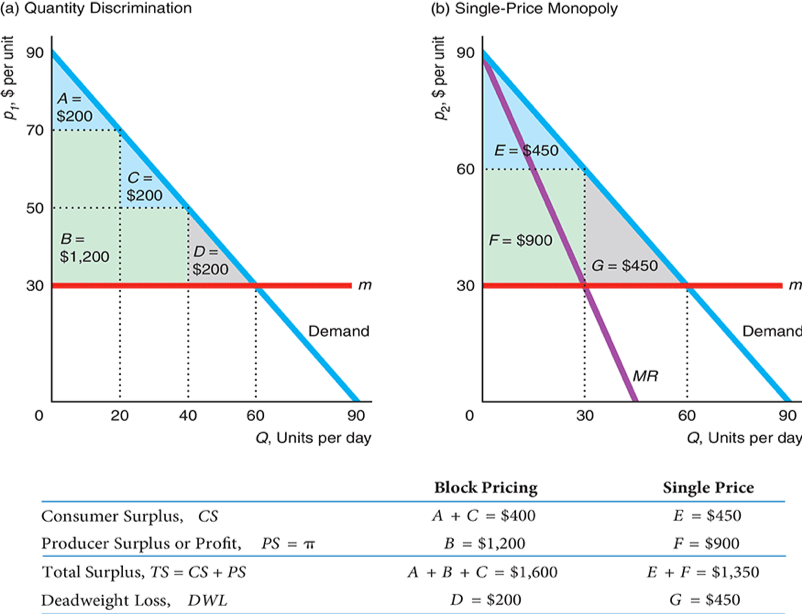
\includegraphics[scale=0.66]{../images/price_disc/block.png}
	\end{figure}
}

\frame{
	\frametitle{Outline}
	\begin{enumerate}
	\item Price Discrimination
	\item[]
	\item Perfect Price Discrimination
	\item[]
	\item Group Price Discrimination
	\item[]
	\item Nonlinear Price Discrimination
	\item[]
	\item \alert{Two-Part Pricing}
	\item[]
	\item Bundling
	\item[]
	\item Peak-Load Pricing
	\item[]
	\item Pricing in Practice
	\end{enumerate}
}

\frame{
	\frametitle{5. Two-Part Pricing}
	\begin{itemize}
	\item With \underline{two-part pricing}, the firm charges each consumer a lump-sum \underline{access fee} for the right to buy as many units of the good as the consumer wants at a per-unit price.
	\item[]
	\item With two-part pricing, a consumer's overall expenditure for an amount $q$ consists of an access fee, $A$, and a per-unit price $p$. So total expenditure is:
		\begin{align*}
		E = A + pq
		\end{align*}
	\item To engage in two-part pricing, a firm must have market power, know how individual demand curves vary across its customers, and be able to prevent resale.
	\end{itemize}
}

\frame{
	\frametitle{5. Two Part Pricing: Identical Consumers}
	\begin{itemize}
	\item With identical consumers, a firm can set a two-part price that is efficient ($p=MC$), and results in all surplus going to the firm ($CS=0$).
	\item[]
	\item In this case, if the firm were to charge $p>MC$, it would sell fewer units and make a smaller profit.
	\end{itemize}
}

\frame{
	\frametitle{5. Two Part Pricing: Identical Consumers}
	\begin{figure}
	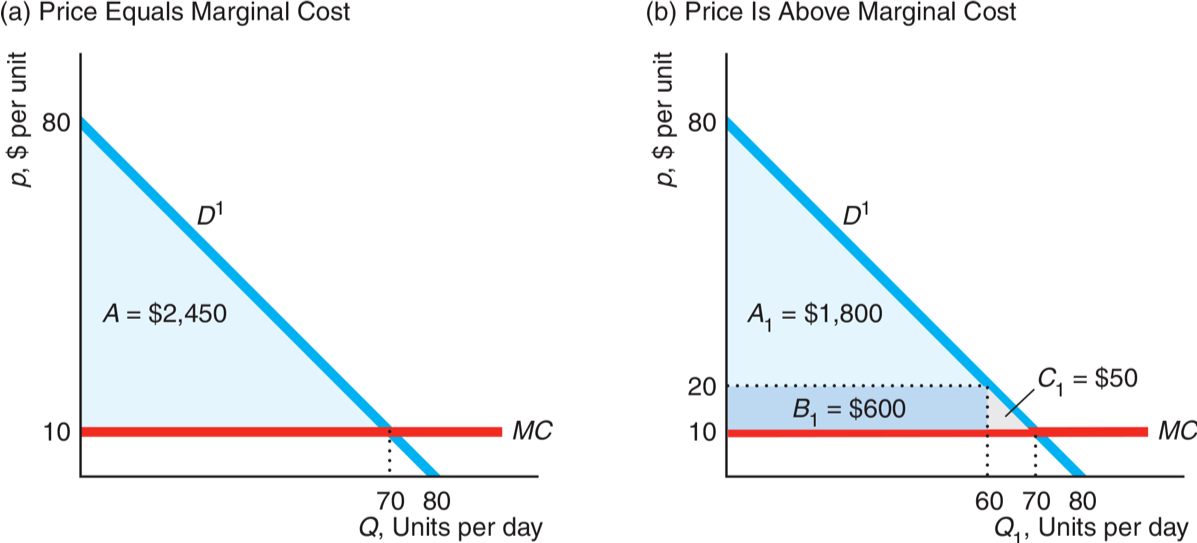
\includegraphics[scale=0.66]{../images/price_disc/two_identical.png}
	\end{figure}
}

\frame{
	\frametitle{5. Two Part Pricing: Heterogeneous Consumers}
	\begin{itemize}
	\item Two-part pricing is more complex if different consumers have different demand curves.
	\item[]
	\item Different demand curves implies consumers have different $CS$.
	\item[]
	\item Two-part pricing would require that the monopolist charge different access fees, and this may not be possible.
	\end{itemize}
}

\frame{
	\frametitle{5. Two Part Pricing: Heterogenous Consumers}
	\begin{figure}
	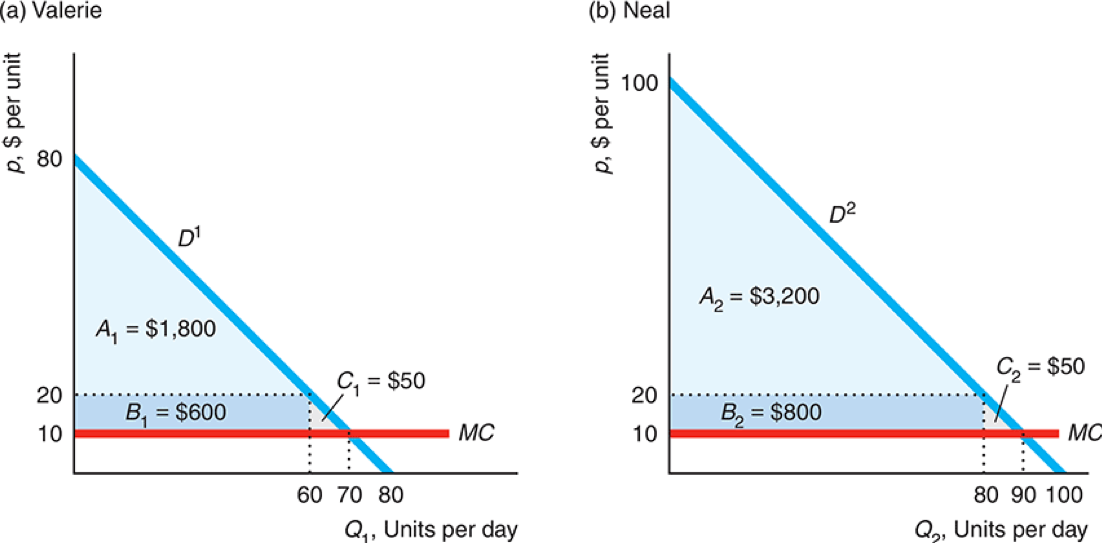
\includegraphics[scale=0.66]{../images/price_disc/two_diff.png}
	\end{figure}
}

\frame{
	\frametitle{Outline}
	\begin{enumerate}
	\item Price Discrimination
	\item[]
	\item Perfect Price Discrimination
	\item[]
	\item Group Price Discrimination
	\item[]
	\item Nonlinear Price Discrimination
	\item[]
	\item Two-Part Pricing
	\item[]
	\item \alert{Bundling}
	\item[]
	\item Peak-Load Pricing
	\item[]
	\item Pricing in Practice
	\end{enumerate}
}

\frame{
	\frametitle{6. Bundling}
	\begin{itemize}
	\item Firms with market power often pursue a pricing strategy called \underline{bundling}, where they sell multiple goods or services at a single price.
	\item[]
	\item Most goods are bundles of many separate parts, but firms may bundle even when there are no production advantages and transaction costs are small.
	\item[]
	\item Bundling allows firms to increase profit by charging different consumers different prices based on their willingness to pay.
	\end{itemize}
}

\frame{
	\frametitle{6. Bundling}
	\begin{itemize}
	\item There are two main forms of bundling:
		\begin{enumerate}
		\item \underline{Pure bundling}: Only a package deal is offered.
		\item[]
		\item \underline{Mixed bundling}: Goods are available as a package or separately.
		\end{enumerate}
	\end{itemize}
}

\frame{
	\frametitle{6. Bundling: Example}
	\begin{itemize}
	\item Classic example of bundling: Corel WordPerfect Office
	\item[]
	\item Corel only sells components as part of a bundle (word processor, spreadsheet program, slideshow program, etc.).
	\item[]
	\item Whether or not this strategy is profitable depends on how reservation prices vary across consumers.
	\item[]
	\item For simplicity, assume the marginal cost of producing an extra copy of any program is essentially zero and fixed costs are negligible so that the firm's revenue equals its profit, and that the firm must charge all customers the same price -- that is, the firm cannot price discriminate.
	\end{itemize}
}

\frame{
	\frametitle{6. Bundling: Pure Bundling}
	\begin{itemize}
	\item Pure bundling increases profits if consumers' reservation prices are \underline{negatively correlated}.
		\begin{itemize}
		\item This occurs when the customer who has the higher reservation price for one product has the lower reservation price for the other product.
		\end{itemize}
	\item[]
	\item Pure bundling is more profitable because the firm captures more of the consumer's potential $CS$ - their reservation price.
	\end{itemize}
}

\frame{
	\frametitle{6. Bundling: Pure Bundling}
	\begin{figure}
	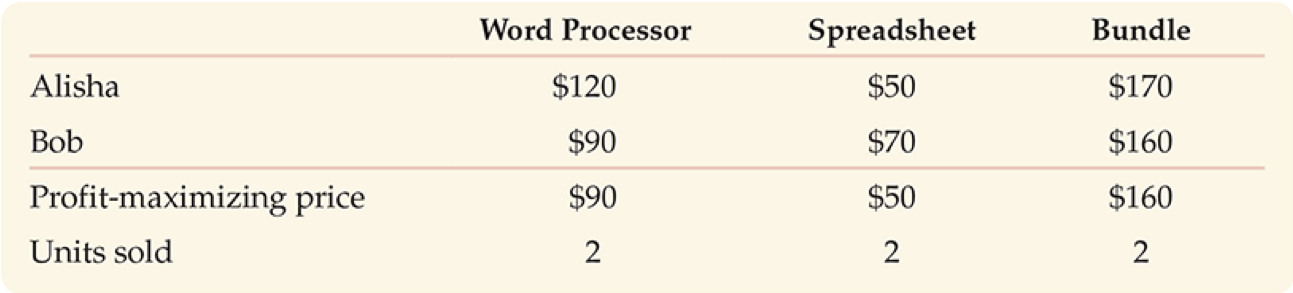
\includegraphics[scale=0.66]{../images/price_disc/pure_bundle.png}
	\caption{Pure Bundling with Negatively Correlated Reservation Prices}
	\end{figure}
}

\frame{
	\frametitle{6. Bundling: Pure Bundling}
	\begin{itemize}
	\item Pure bundling decreases profits if reservation prices are \underline{positively correlated}.
		\begin{itemize}
		\item This occurs when the customer who has the highest reservation price for one product also has the highest reservation price for the other product.
		\end{itemize}
	\end{itemize}
}

\frame{
	\frametitle{6. Bundling: Pure Bundling}
	\begin{figure}
	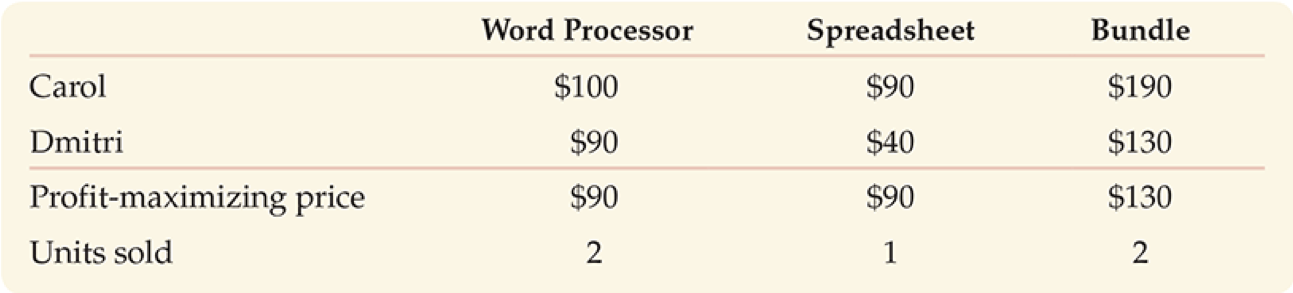
\includegraphics[scale=0.66]{../images/price_disc/pure_bundle_pos.png}
	\caption{Pure Bundling with Positively Correlated Reservation Prices}
	\end{figure}
}

\frame{
	\frametitle{6. Bundling: Mixed Bundling}
	\begin{itemize}
	\item With mixed bundling, consumers are allowed to buy the pure bundle, or to buy any of the bundle's components separately.
	\item[]
	\item As an example, let's revisit the software example.
	\end{itemize}
}

\frame{
	\frametitle{6. Bundling: Mixed Bundling}
	\begin{figure}
	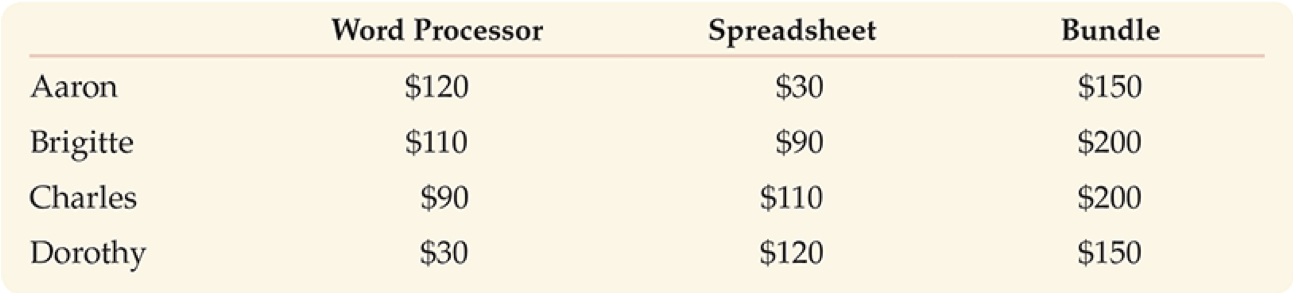
\includegraphics[scale=0.66]{../images/price_disc/mixed_bundle.png}
	\end{figure}
}

\frame{
	\frametitle{6. Bundling}
	\begin{itemize}
	\item Another form of bundling: \underline{Tie in sales}
	\item[]
	\item Tie in sales require customers who buy one product from a firm to make all concurrent and subsequent purchases of a related product from that firm.
	\item[]
	\item Tie in requirement allows the firm to identify heavy users and charge them more per unit.
	\item[]
	\item Example: Printer manufacturers.
		\begin{itemize}
		\item If the firm can require that consumers buy their ink cartridges from them, the firm will be able to capture most of the consumers' surplus. Heavy users pay more than light users due to the high cost of ink cartridges.
		\item Manufacturers of printers (such as HP) use strategies (such as design of warranty) to encourage use of new brand-name cartridges and not to refill them.
		\end{itemize}
	\end{itemize}
}

\frame{
	\frametitle{Outline}
	\begin{enumerate}
	\item Price Discrimination
	\item[]
	\item Perfect Price Discrimination
	\item[]
	\item Group Price Discrimination
	\item[]
	\item Nonlinear Price Discrimination
	\item[]
	\item Two-Part Pricing
	\item[]
	\item Bundling
	\item[]
	\item \alert{Peak-Load Pricing}
	\item[]
	\item Pricing in Practice
	\end{enumerate}
}

\frame{
	\frametitle{7. Peak-Load Pricing}
	\begin{itemize}
	\item \underline{Peak-load Pricing}: Charge higher prices during periods of peak demand than in other periods.
	\item[]
	\item Commonly used by firms that face capacity constraints (e.g. hotels, airlines, utilities).
		\begin{itemize}
		\item During peak demand period, the firm sets a high price to limit demand to available capacity.
		\item During low demand period, profit maximizing price leaves excess capacity.
		\end{itemize}
	\end{itemize}
}

\frame{
	\frametitle{7. Peak-Load Pricing}
	\begin{figure}
	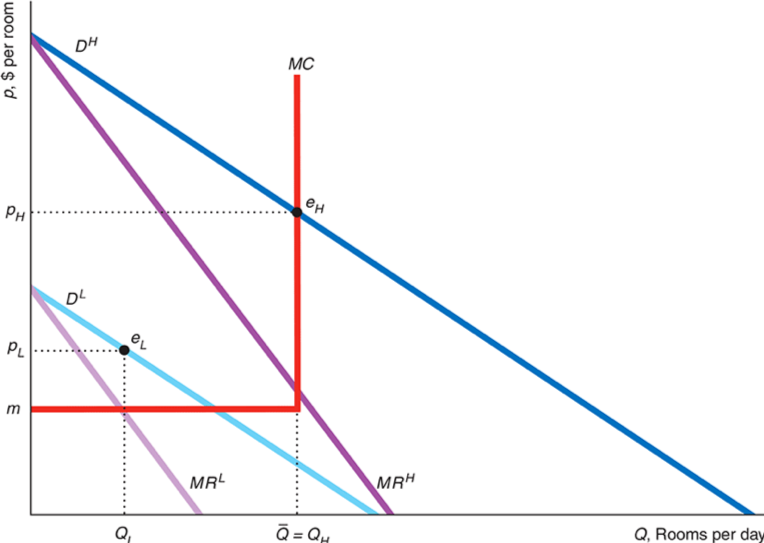
\includegraphics[scale=0.66]{../images/price_disc/peak.png}
	\end{figure}
}

\frame{
	\frametitle{Outline}
	\begin{enumerate}
	\item Price Discrimination
	\item[]
	\item Perfect Price Discrimination
	\item[]
	\item Group Price Discrimination
	\item[]
	\item Nonlinear Price Discrimination
	\item[]
	\item Two-Part Pricing
	\item[]
	\item Bundling
	\item[]
	\item Peak-Load Pricing
	\item[]
	\item \alert{Pricing in Practice}
	\end{enumerate}
}

\frame{
	\frametitle{8. Pricing in Practice: Whistler-Blackcomb}
	\begin{itemize}
	\item Price discrimination, two-part pricing, bundling, and peak-load pricing are not mutually exclusive.
	\item[]
	\item Firms often use all four pricing tools simultaneously.
	\item[]
	\item E.g. Whistler Blackcomb Ski Resort.
	\end{itemize}
}

\frame{
	\frametitle{8. Pricing in Practice: Whistler-Blackcomb}
	\begin{itemize}
	\item Whistler satisfies three conditions needed to apply tools:
		\begin{enumerate}
		\item Has considerable \textit{market power} as a top ski destination.
		\item[]
		\item Obtains extensive \textit{information} about customers by tracking skiing habits.
		\item[]
		\item Prevents \textit{resale} of discount tickets (season pass/multi-day ticket) by putting photo on pass.
		\end{enumerate}
	\end{itemize}
}

\frame{
	\frametitle{8. Pricing in Practice: Whistler-Blackcomb}
	\begin{itemize}
	\item Whistler-Blackcomb:
		\begin{itemize}
		\item engages in individual price discrimination based on an individual's skiing history.
			\begin{itemize}
			\item By tracking skiing history and linking it to the customer's personal address, the company is able to send personalized promotions to customers.
			\end{itemize}
		\item engages in nonlinear price discrimination by offering discounts for multi-day passes or groups.
		\item engages in group price discrimination by setting different prices by age.
		\item utilizes two-part pricing. Local residents can buy an access pass that allows them to pay lower daily prices in season.
		\item utilizes bundling by combining lift tickets with rentals/lessons.
		\item engages in peak load pricing by varying fees over week/season.
		\end{itemize}
	\end{itemize}
}

\frame{
	\frametitle{Takeaways}
	\begin{enumerate}
	\item Firms that have market power, information about consumer demand, and are able to prevent resale can engage in price discrimination.
	\item[]
	\item Price discrimination allows the firm to capture some (or all) consumer surplus.
	\item[]
	\item Two-part pricing, bundling, and peak-load pricing can also increase the profitability of a firm with market power.
	\end{enumerate}
}

\end{document}

